%%%% fatec-article.tex, 2024/03/10

\documentclass[
  a4paper,%% Tamanho de papel: a4paper, letterpaper (^), etc.
  12pt,%% Tamanho de fonte: 10pt (^), 11pt, 12pt, etc.
  english,%% Idioma secundário (penúltimo) (>)
  brazilian,%% Idioma primário (último) (>)
]{article}

%% Pacotes utilizados
\usepackage[]{fatec-article}

%% Início do documento
\begin{document}
\vspace{8cm}
\begin{center}
    \large \textbf{\title{ARTEFATOS DO PROJETO DE SOFTWARE}}
\end{center}

\maketitle

\break

\tableofcontents

\break


%exemplo da forma de organização das seções e subseções, você deverá adaptar o template para a realidade do seu projeto.


    
    \section*{Diagrama de Caso de Uso}
    \addcontentsline{toc}{section}{Diagrama de Caso de Uso}

    Atores: 

    Proprietário: Usuário responsável pela administração do sistema, incluindo o acesso e o cadastro de fazendas.

    Agricultor: Usuário que interage diretamente com o sistema para obter diagnósticos sobre as plantas, registrar imagens, consultar históricos e analisar probabilidades baseadas em dados históricos.

    O proprietário deve realizar o login no sistema e cadastrar a fazenda.



            \begin{figure}[h]
\centering
\caption{Diagrama de caso de uso}%
\label{fig:diagrama-caso-uso}
 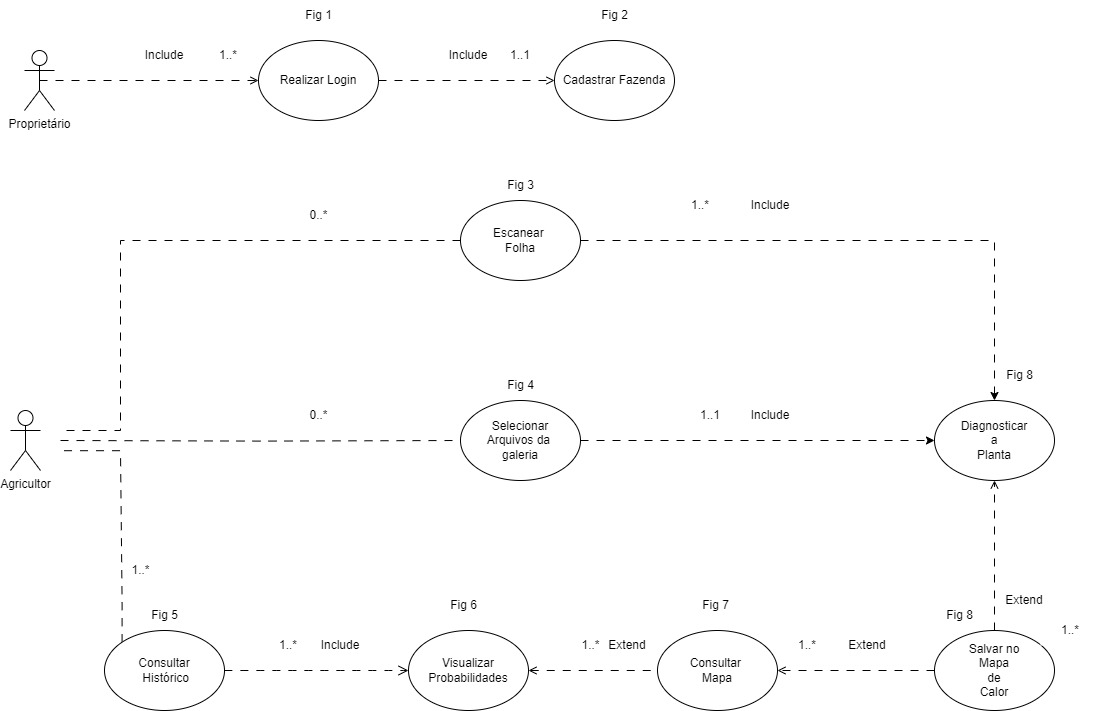
\includegraphics[width=1.1\textwidth]{Logos/Caso_uso_solo - Copia.jpg}
\SourceOrNote{Autoria Própria (2024)}
\end{figure}

\newpage

O agricultor pode escanear uma folha para obter o diagnóstico dela. Além disso, ele tem a opção de salvar a imagem no mapa de calor. Na funcionalidade "Selecionar Arquivos da Galeria", o agricultor pode usar uma foto já armazenada em seu celular para realizar o diagnóstico. O agricultor também pode consultar o histórico de diagnósticos anteriores e visualizar as probabilidades relacionadas a partir desse histórico.
    
Por fim, o agricultor pode salvar a imagem escaneada no mapa de calor, onde ela ficará registrada juntamente com a localização geográfica de onde a foto foi tirada.

\section*{Diagrama de Redes}
\addcontentsline{toc}{section}{Diagrama de Redes}

    Um diagrama de redes é uma representação visual que ilustra a estrutura e as interconexões entre diferentes elementos ou componentes de um sistema, como nós e conexões em uma rede. Ele é utilizado para mostrar como os recursos, como informações, dispositivos ou processos, estão organizados e se comunicam dentro de um ambiente.
  
    \begin{figure}[h]
        \centering
        \caption{Diagrama de Redes}%
        \label{fig:diagrama-redes}
         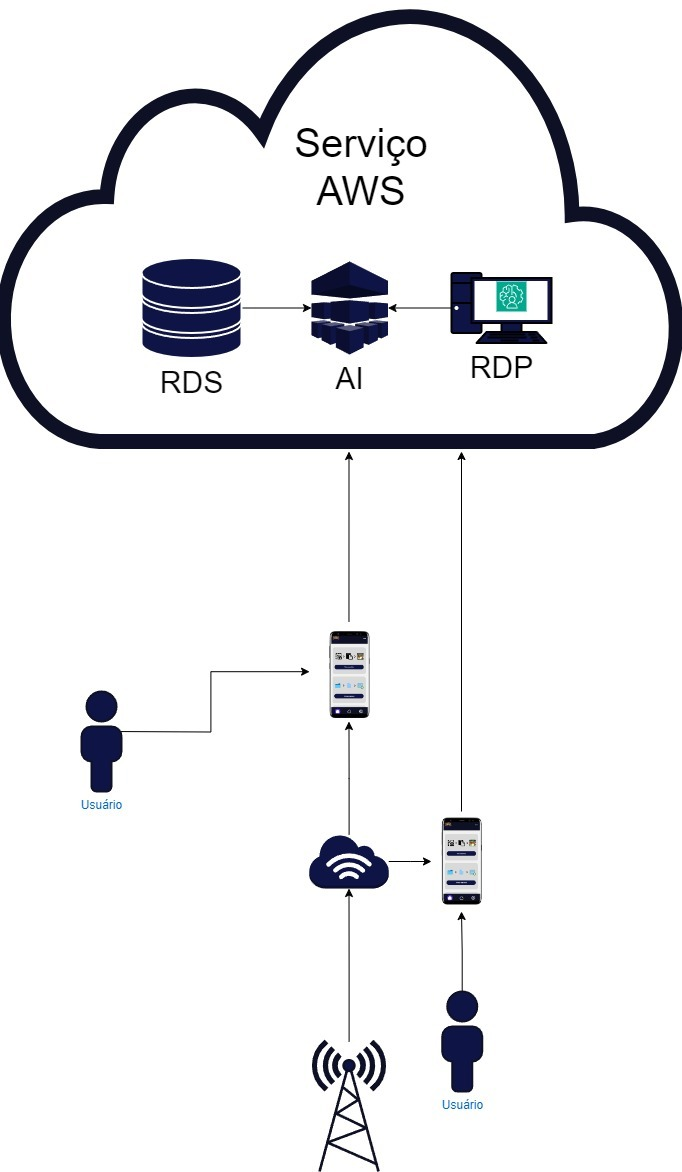
\includegraphics[width=0.5\textwidth]{Logos/Diagrama_redes.jpg}
        \SourceOrNote{Autoria Própria (2024)}
        \end{figure}

        \newpage

        No diagrama de redes é possível identificar que o usuário se conecta com a internet e acessa o serviço AWS onde fica localizada a RDP (maquina virtual da AWS) e o RDS (O banco de dados para treinar a IA).

        \section*{MODELO DE NEGÓCIOS CANVAS}
        \addcontentsline{toc}{section}{Modelo de Negócios Canvas}

        Por meio do Canvas, foi possível facilitar o planejamento e a compreensão do projeto, aprimorando a clareza e proporcionando uma visão mais eficaz de como estruturar a criação do projeto.

        \begin{figure}[h]
            \centering
            \caption{Diagrama de caso de uso}%
            \label{fig:canvas}
             \includegraphics[width=1.1\textwidth]{Logos/Canva.jpg}
            \SourceOrNote{Autoria Própria (2024)}
            \end{figure}

            \newpage

            \section*{Modelagem de Banco de Dados}
    
            \addcontentsline{toc}{section}{Modelagem Banco de Dados}

            \subsection*{Modelagem Conceitual}
            A modelagem conceitual foi criada para facilitar o entendimento dos processos, no qual seria salva as informações de uso de cada usuário e observar como funciona o banco de dados de uma maneira mais ampla do projeto, afim de facilitar a criação futuramente.

                \begin{figure}[h]
                \centering
                \caption{Modelagem Conceitual}%
                \label{fig:mod-conceitual}
                 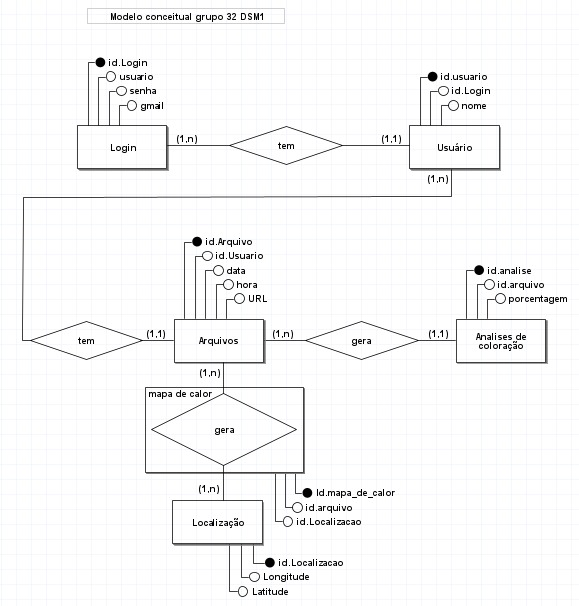
\includegraphics[width=0.6\textwidth]{Logos/BDC.jpeg}
                \SourceOrNote{Autoria Própria (2024)}
                \end{figure}

                \newpage

                O banco de dados desempenha um papel fundamental na gestão das informações, sendo essencial para armazenar, organizar e recuperar dados
                .
                \subsection*{Modelagem Lógica}
     
                    \begin{figure}[h]
                    \centering
                    \caption{Modelagem Lógica}%
                    \label{fig:mod-logica}
                     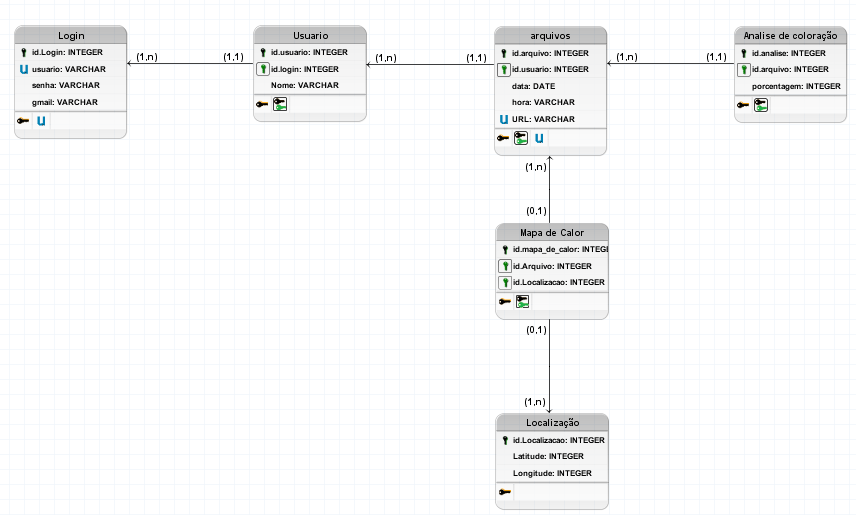
\includegraphics[width=1.1\textwidth]{Logos/mod_logic1.png}
                    \SourceOrNote{Autoria Própria (2024)}
                    \end{figure}

                   

                    O modelo lógico de um banco de dados serve para organizar as informações, definindo como os dados serão armazenados e quais serão os tipos de suas variáveis, afim de deixar mais claro o funionamento do banco de dados e o entendimento de como cada atributo será armazenado.


                \section*{Diário de Bordo}
                \addcontentsline{toc}{section}{Diário de Bordo}

                    \begin{figure}[h]
                    \centering
                    \caption{Diário de Bordo}%
                    \label{fig:D-bordo1}
                     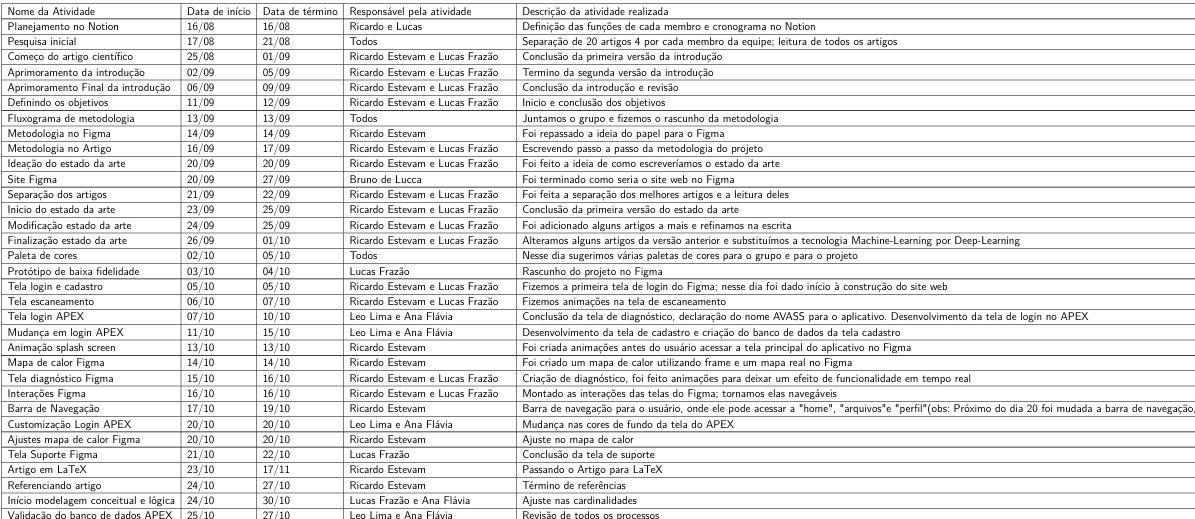
\includegraphics[width=1.1\textwidth]{Logos/loog_book1.png}
                    \SourceOrNote{Autoria Própria (2024)}
                    \end{figure}

                    \newpage
                    
                    \begin{figure}[h]
                        \centering
                        \caption{Diário de Bordo}%
                        \label{fig:D-bordo2}
                         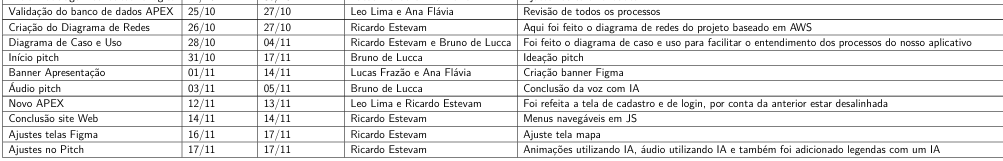
\includegraphics[width=1.1\textwidth]{Logos/loog_book2.png}
                        \SourceOrNote{Autoria Própria (2024)}
                        \end{figure}

                        \newpage
           
    
                    

\end{document}